\documentclass[twocolumn]{article}

\def\bibsection{\section*{References}}
\usepackage[style=nature, backend=biber]{biblatex}
\addbibresource{refs.bib}

\usepackage[utf8]{inputenc}
\usepackage{listings}
\usepackage{color} %red, green, blue, yellow, cyan, magenta, black, white
\definecolor{mygreen}{RGB}{0,0.6,0} % color values Red, Green, Blue
\definecolor{mygray}{RGB}{0.47,0.47,0.33}
\definecolor{myorange}{RGB}{0.8,0.4,0}
\definecolor{mywhite}{RGB}{0.98,0.98,0.98}
\definecolor{myblue}{RGB}{0.01,0.61,0.98}
\usepackage{graphicx}
\usepackage{etoolbox}
\usepackage[normalem]{ulem}    
\usepackage{tikz}
\usepackage{float}
\usepackage{subcaption}
\usetikzlibrary{shapes.geometric, intersections, patterns}
\usepackage{pgf, pgfcore, pgfplots, pgfplotstable}
\usepgfplotslibrary{fillbetween}
\pgfplotsset{compat=newest}

\newcommand{\rpm}{\raisebox{.2ex}{$\scriptstyle\pm$}}

%% https://tex.stackexchange.com/questions/211415/how-to-set-up-listings-for-use-code-from-arduino
\newcommand*{\FormatDigit}[1]{\ttfamily\textcolor{mygreen}{#1}}
%% https://tex.stackexchange.com/questions/32174/listings-package-how-can-i-format-all-numbers
\lstdefinestyle{FormattedNumber}{%
	literate=*{0}{{\FormatDigit{0}}}{1}%
	{1}{{\FormatDigit{1}}}{1}%
	{2}{{\FormatDigit{2}}}{1}%
	{3}{{\FormatDigit{3}}}{1}%
	{4}{{\FormatDigit{4}}}{1}%
	{5}{{\FormatDigit{5}}}{1}%
	{6}{{\FormatDigit{6}}}{1}%
	{7}{{\FormatDigit{7}}}{1}%
	{8}{{\FormatDigit{8}}}{1}%
	{9}{{\FormatDigit{9}}}{1}%
	{.0}{{\FormatDigit{.0}}}{2}% Following is to ensure that only periods
	{.1}{{\FormatDigit{.1}}}{2}% followed by a digit are changed.
	{.2}{{\FormatDigit{.2}}}{2}%
	{.3}{{\FormatDigit{.3}}}{2}%
	{.4}{{\FormatDigit{.4}}}{2}%
	{.5}{{\FormatDigit{.5}}}{2}%
	{.6}{{\FormatDigit{.6}}}{2}%
	{.7}{{\FormatDigit{.7}}}{2}%
	{.8}{{\FormatDigit{.8}}}{2}%
	{.9}{{\FormatDigit{.9}}}{2}%
	%{,}{{\FormatDigit{,}}{1}% depends if you want the "," in color
	{\ }{{ }}{1}% handle the space
	,%
}


\lstset{%
	backgroundcolor=\color{mywhite},   
	basicstyle=\footnotesize,       
	breakatwhitespace=false,         
	breaklines=true,                 
	captionpos=b,                   
	commentstyle=\color{red},    
	deletekeywords={...},           
	escapeinside={\%*}{*)},          
	extendedchars=true,              
	frame=shadowbox,                    
	keepspaces=true,                 
	keywordstyle=\color{myorange},       
	language=Octave,                
	morekeywords={*,...},            
	numbers=left,                    
	numbersep=5pt,                   
	numberstyle=\tiny\color{mygray}, 
	rulecolor=\color{black},         
	rulesepcolor=\color{myblue},
	showspaces=false,                
	showstringspaces=false,          
	showtabs=false,                  
	stepnumber=2,                    
	stringstyle=\color{myorange},    
	tabsize=2,                       
	title=\lstname,
	emphstyle=\bfseries\color{blue},%  style for emph={} 
}    

%% language specific settings:
\lstdefinestyle{Arduino}{%
	style=FormattedNumber,
	keywords={void},%                 define keywords
	morecomment=[l]{//},%             treat // as comments
	morecomment=[s]{/*}{*/},%         define /* ... */ comments
	emph={HIGH, OUTPUT, LOW},%        keywords to emphasize
}

\newtoggle{InString}{}% Keep track of if we are within a string
\togglefalse{InString}% Assume not initally in string

\newcommand{\classname}{EE3: Introduction to Electrical Engineering}
\newcommand{\project}{- Path Following Robot -}
\newcommand{\authorname}{Brian Dionigi Raymond\\Kevin Ke-En Sun}
\newcommand{\instructor}{Prof. Briggs}

\newcommand{\sectionTitle}[1]{ {\large\textbf{\uline{#1}}} \\ \vspace{1.5em} }
\newcommand{\subsectionTitle}[1]{ {\hspace{2em}\uline{#1}} \\ \vspace{1em} }

\newcommand{\textIntroOne}{The goal of the project was to design a car able to follow a path represented by a black line on a white background. The car uses three sensors to detect where to go on the path, one each on the front, right, and left. The sensors work by using an IR LED that reflects IR light off the ground and into a phototransistor. They are connected to each other as shown in Figure \ref{fig:circuitSensors}. A phototransistor works like a transistor which is like a switch. A transistor has three terminals: a base, emitter and collector. When a voltage is applied to the base that is relatively higher than the voltage on the emitter, current flows from the emitter to the collector. On the other hand, if the voltage applied to the base is relatively lower than the voltage on the emitter, then no current flows. A phototransistor is different from a regular transistor, however, in that the base is sensitive to light as opposed to voltage. When light is shown on the base, current flows, but if there is no light, there is no current. An emitter follower setup was used for the sensors (signal response is low in absence of IR light and high in its presence). See Figure \ref{fig:circuitMotors} for the proper wiring.}

\newcommand{\textIntroTwo}{The car's motion is controlled by going straight whenever the front sensor triggers low. As soon as either the left or right sensors trigger low, the car turns in the opposite direction (left if right triggers, right if left triggers) until the front sensor trigger again triggers low again. The rate at which the car turns back towards the front sensor was adjusted using PID methods\cite{beauregard_2011} to allow the car to orient itself along the line both faster and more precisely. After the front sensor triggers low, the car would then continue straight again until it finds the stopping condition (black lines perpendicular to the track). Pulse width modulation (PWM) and transistors are used in conjunction to control the speed of the motor. The PWM signal is connected to the base of the transistor and the duty cycle of the PWM is used to control the speed of the motor. Increasing the duty cycle of the PWM increases the speed of the motor by increasing the relative time for which the motor is on to that for which it is turned off. LEDs are used to signal which direction the car is going: a green LED signals forward, a red LED signals left, and a blue LED signals right. In the case of the car’s stopping conditions being met, both the blue and red LEDs turn on. LEDs have two sides: a negative (`n’) side and a positive (`p’) side. The n side is filled with electrons and the p side is filled with holes. Energy is released when electrons annihilate the holes and this energy is most likely released in the form of light.
}
\newcommand{\textTestDesign}{To obtain a comprehensive test of our path sensing subsystem and sensors, we took a multi step approach involving testing the initial, adjusted, and mapped readings from our getDistance() function before testing the entire function. Each of our tests involved a setup where the robot was propped onto a cardboard jack (e.g. paper roll) and the sensors suspended over a stationary piece of paper that was unmarked besides lines acting as a metric ruler. Using another similarly delineated paper with a $2cm$-wide black line approximating that on the course, we aimed to simulate the robot’s motion by moving the line from to different distances from each of the sensors.
}
\newcommand{\textTestConduction}{The test was conducted in four parts. For the first three parts which consisted of the function component tests, we took measurements for each of the sensors separately, centering them on the black line, and measured \rpm$1cm$ from the edge of the line. Originally, we measured \rpm$2cm$ but noticed that past a centimeter made no difference as the IR phototransistor was unable to read that far away. From these three trials, we were able to tune our processing of the sensor readings to better gauge the distance. Then for the final trial where we tested the overall getDistance() function, we took measurements by starting (\rpm$4cm$) from the front sensor and taking measurements of the estimated distance at $0.25cm$ intervals going back to the center.
}
\newcommand{\textTestAnalysis}{After each of our trials, we graphed the estimated distance (function’s output printed to Serial) versus the actual distance (as measured). The first trial (raw sensor readings vs. distance as measured) gave us a polynomial graph so we found the polynomial regression and solved in terms y in order to obtain a distance value from the sensor reading. Taking new measurements using our newly found formulas gave us the second trial, where after graphing we noticed our global minima were preserved but the range condensed to not contain the entire range of \rpm$1cm$ that we knew the sensors could read from Trial 1. Having adjusted our code once more before our final trial, we moved onto the fourth and final trial, where we graphed all of the sensors on the same axis with $x=0$ being the center of the front sensor. From here we began our interpretation of the results.
}
\newcommand{\textTestInterpretation}{Looking at the trial of the overall performance of the getDistance() function, performance was interpreted according to two metrics: absolute error at different point and overall trend. For the sensor function to be acceptable, the distance should decrease as the black line goes from either side sensor towards the front sensor and reach a minimum once at the direct sensor of the car. In addition to this, we judged success on the difference between the estimated distance and the actual distance. As the sensor an only read a maximum of 1cm away, we aimed for a maximum error of half that or 0.5cm.
}
\newcommand{\textTestDiscussion}{Test Discussion plaintext - To be added}
\newcommand{\textRaceResults}{Results Discussion Conduction plaintext - To be added}
\newcommand{\textConclusions}{Conclusions plaintext - To be added}
\newcommand{\textFutureWork}{Future Work plaintext - To be added}
\newcommand{\textReferences}{References plaintext - To be added}

\begin{document}
		
	\begin{center}
		{\LARGE \textsc{\classname \\ \project} \\ \vspace{4pt}}
		\rule[13pt]{0.5\textwidth}{1pt} \\ %\vspace{150pt}
		{\authorname \\ \vspace{2pt}
			Instructor: \instructor \\ \vspace{2pt}
			\today \\ \vspace{2pt}
		}
	\end{center}	
	
	\begin{flushleft}
		\sectionTitle{Introduction}
		
		\textIntroOne \\ \vspace{1em}
		
		\begin{figure}[!h]

			\centering{\textbf{Circuits for Path Sensing and Movement}\par\medskip}
			{\begin{subfigure}[b]{0.45\textwidth}
				\frame{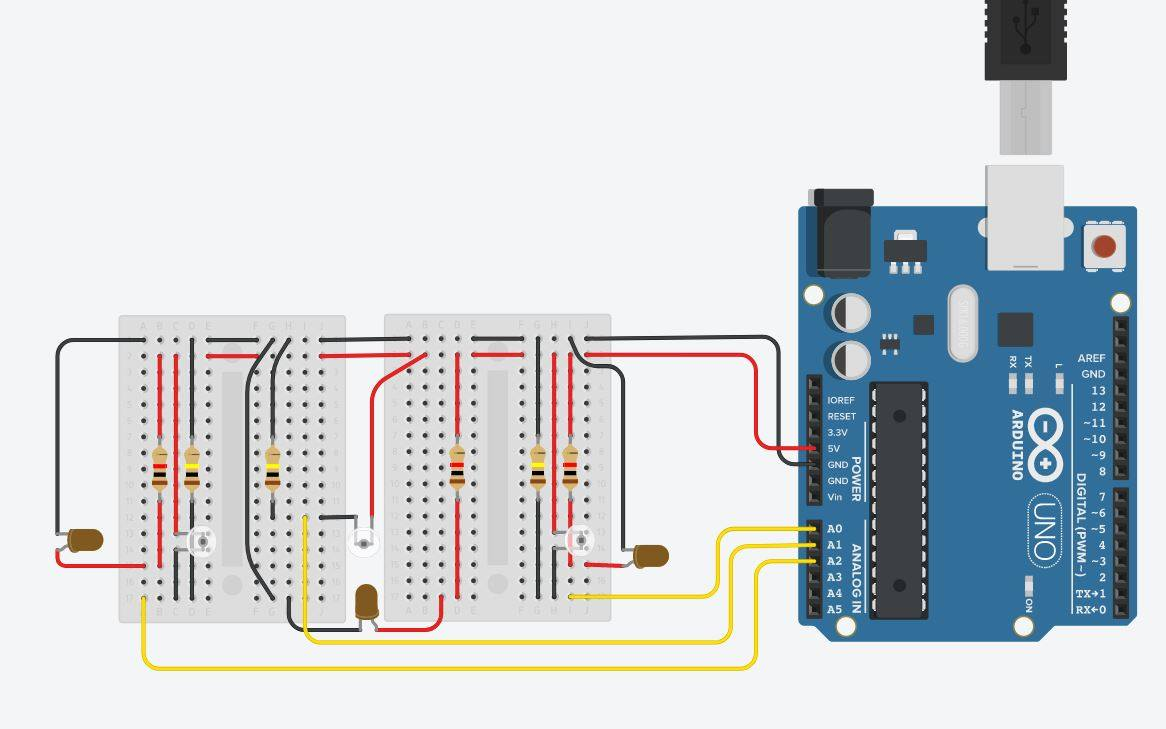
\includegraphics[width=1\columnwidth, keepaspectratio]{CircuitSensors.jpg}}
				\caption{IR LED and Phototransistor Circuit}
				\label{fig:circuitSensors}
			\end{subfigure}\\ \vspace{1em}%
			\begin{subfigure}[b]{0.45\textwidth}
				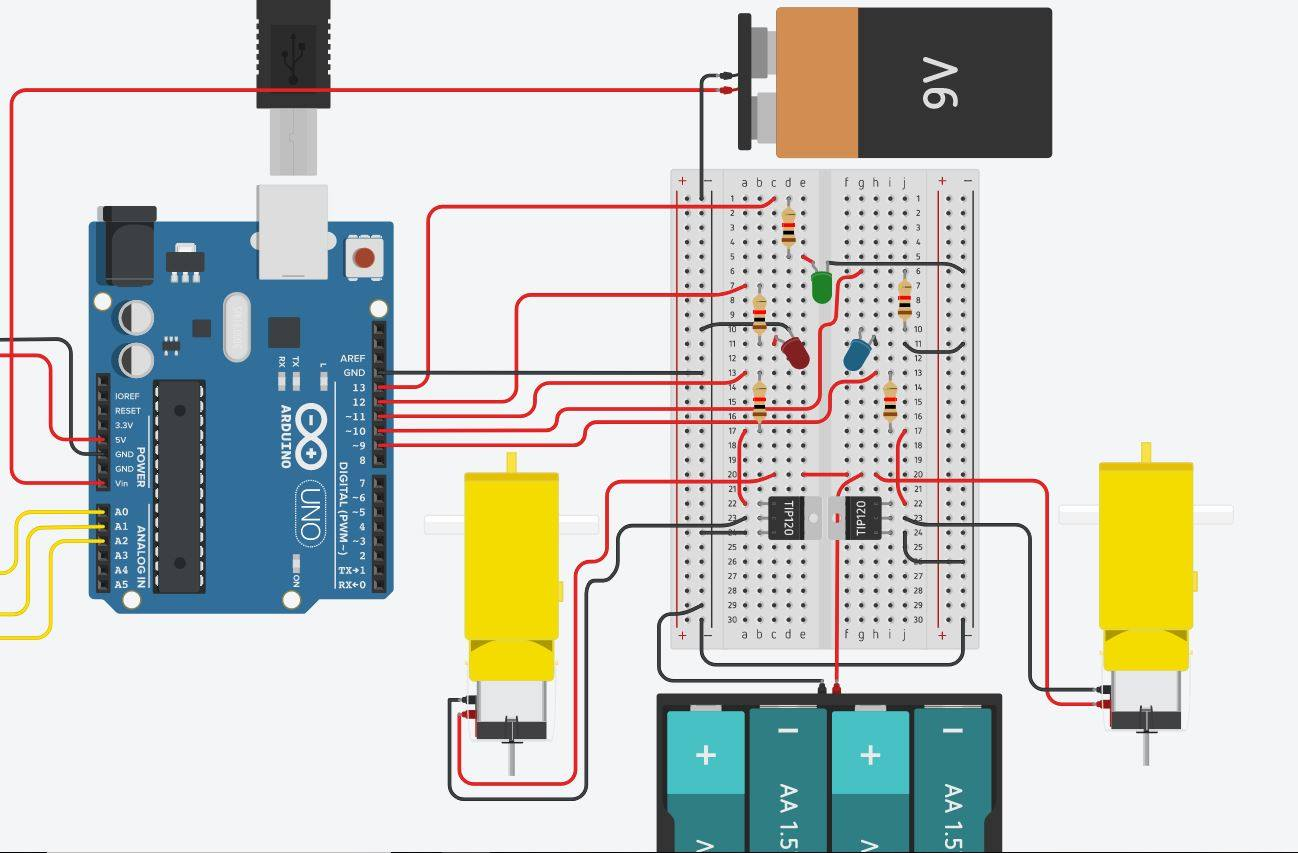
\includegraphics[width=1\columnwidth, keepaspectratio]{CircuitMotors.jpg}
				\caption{Motor and LED Circuit}
				\label{fig:circuitMotors}
			\end{subfigure}
			
			\caption{Circuit schematics for our path following car. In Figure \ref{fig:circuitSensors}, the $1k$ resistors attached to the IR LEDs between the $V_{in}$ and anode ($+$) as well as $10k$ resistors attached to the photo transistors between the emitter and ground. The phototransistors go to Analog pins since their data is transmitted as an analog signal ranging from $0-1000 (arb.)$. In Figure \ref{fig:circuitMotors}, the LEDs are wiring the same way as the IR LEDs from before. The TIP120 is connected to $V_{in}$ through a $1k$ resistor on it's base, to the motor through it's collector, and to ground through it's emitter.}
}
		\end{figure}
		
		\textIntroTwo \\ \vspace{1em}
		
		\sectionTitle{Testing Methodology}
		
		\subsectionTitle{How We Designed the Test}

		\textTestDesign \\ \vspace{1em}
		
		\begin{figure}[!H]
			
			\centering{\textbf{Circuits for Path Sensing and Movement}\par\medskip}
			{\begin{subfigure}[b]{0.45\textwidth}
					\frame{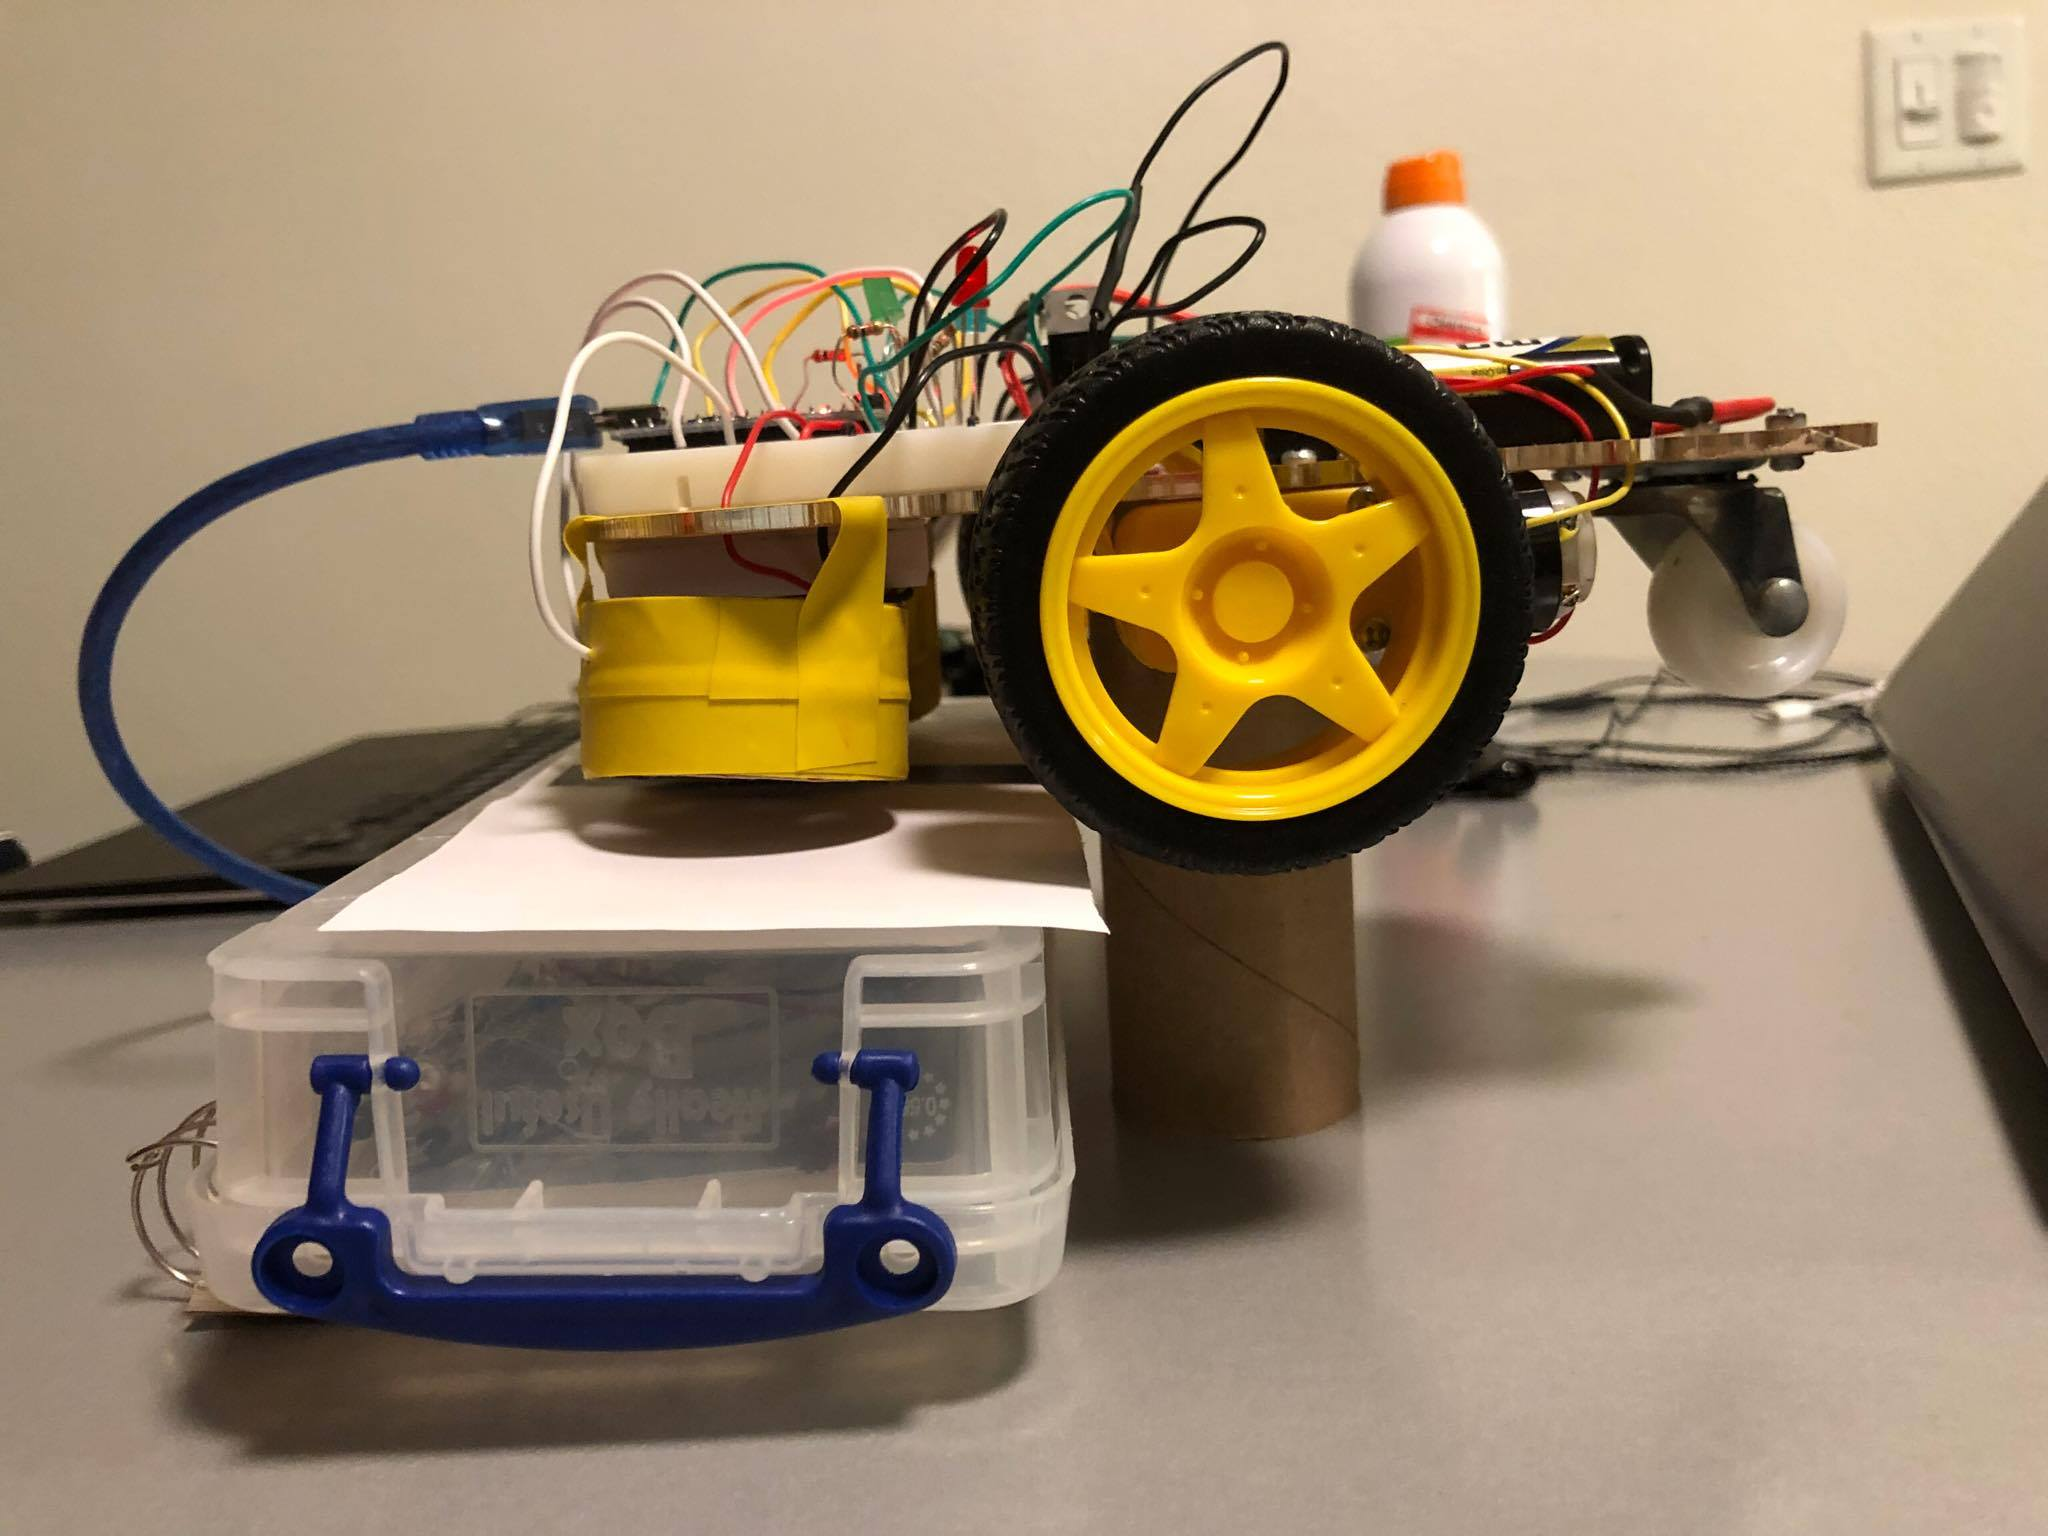
\includegraphics[width=1\columnwidth, keepaspectratio]{TestProcedure_Rig.jpg}}
					\caption{Cardboard Jack}
					\label{fig:procedureRig}
				\end{subfigure}\\ \vspace{1em}%
				\begin{subfigure}[b]{0.45\textwidth}
					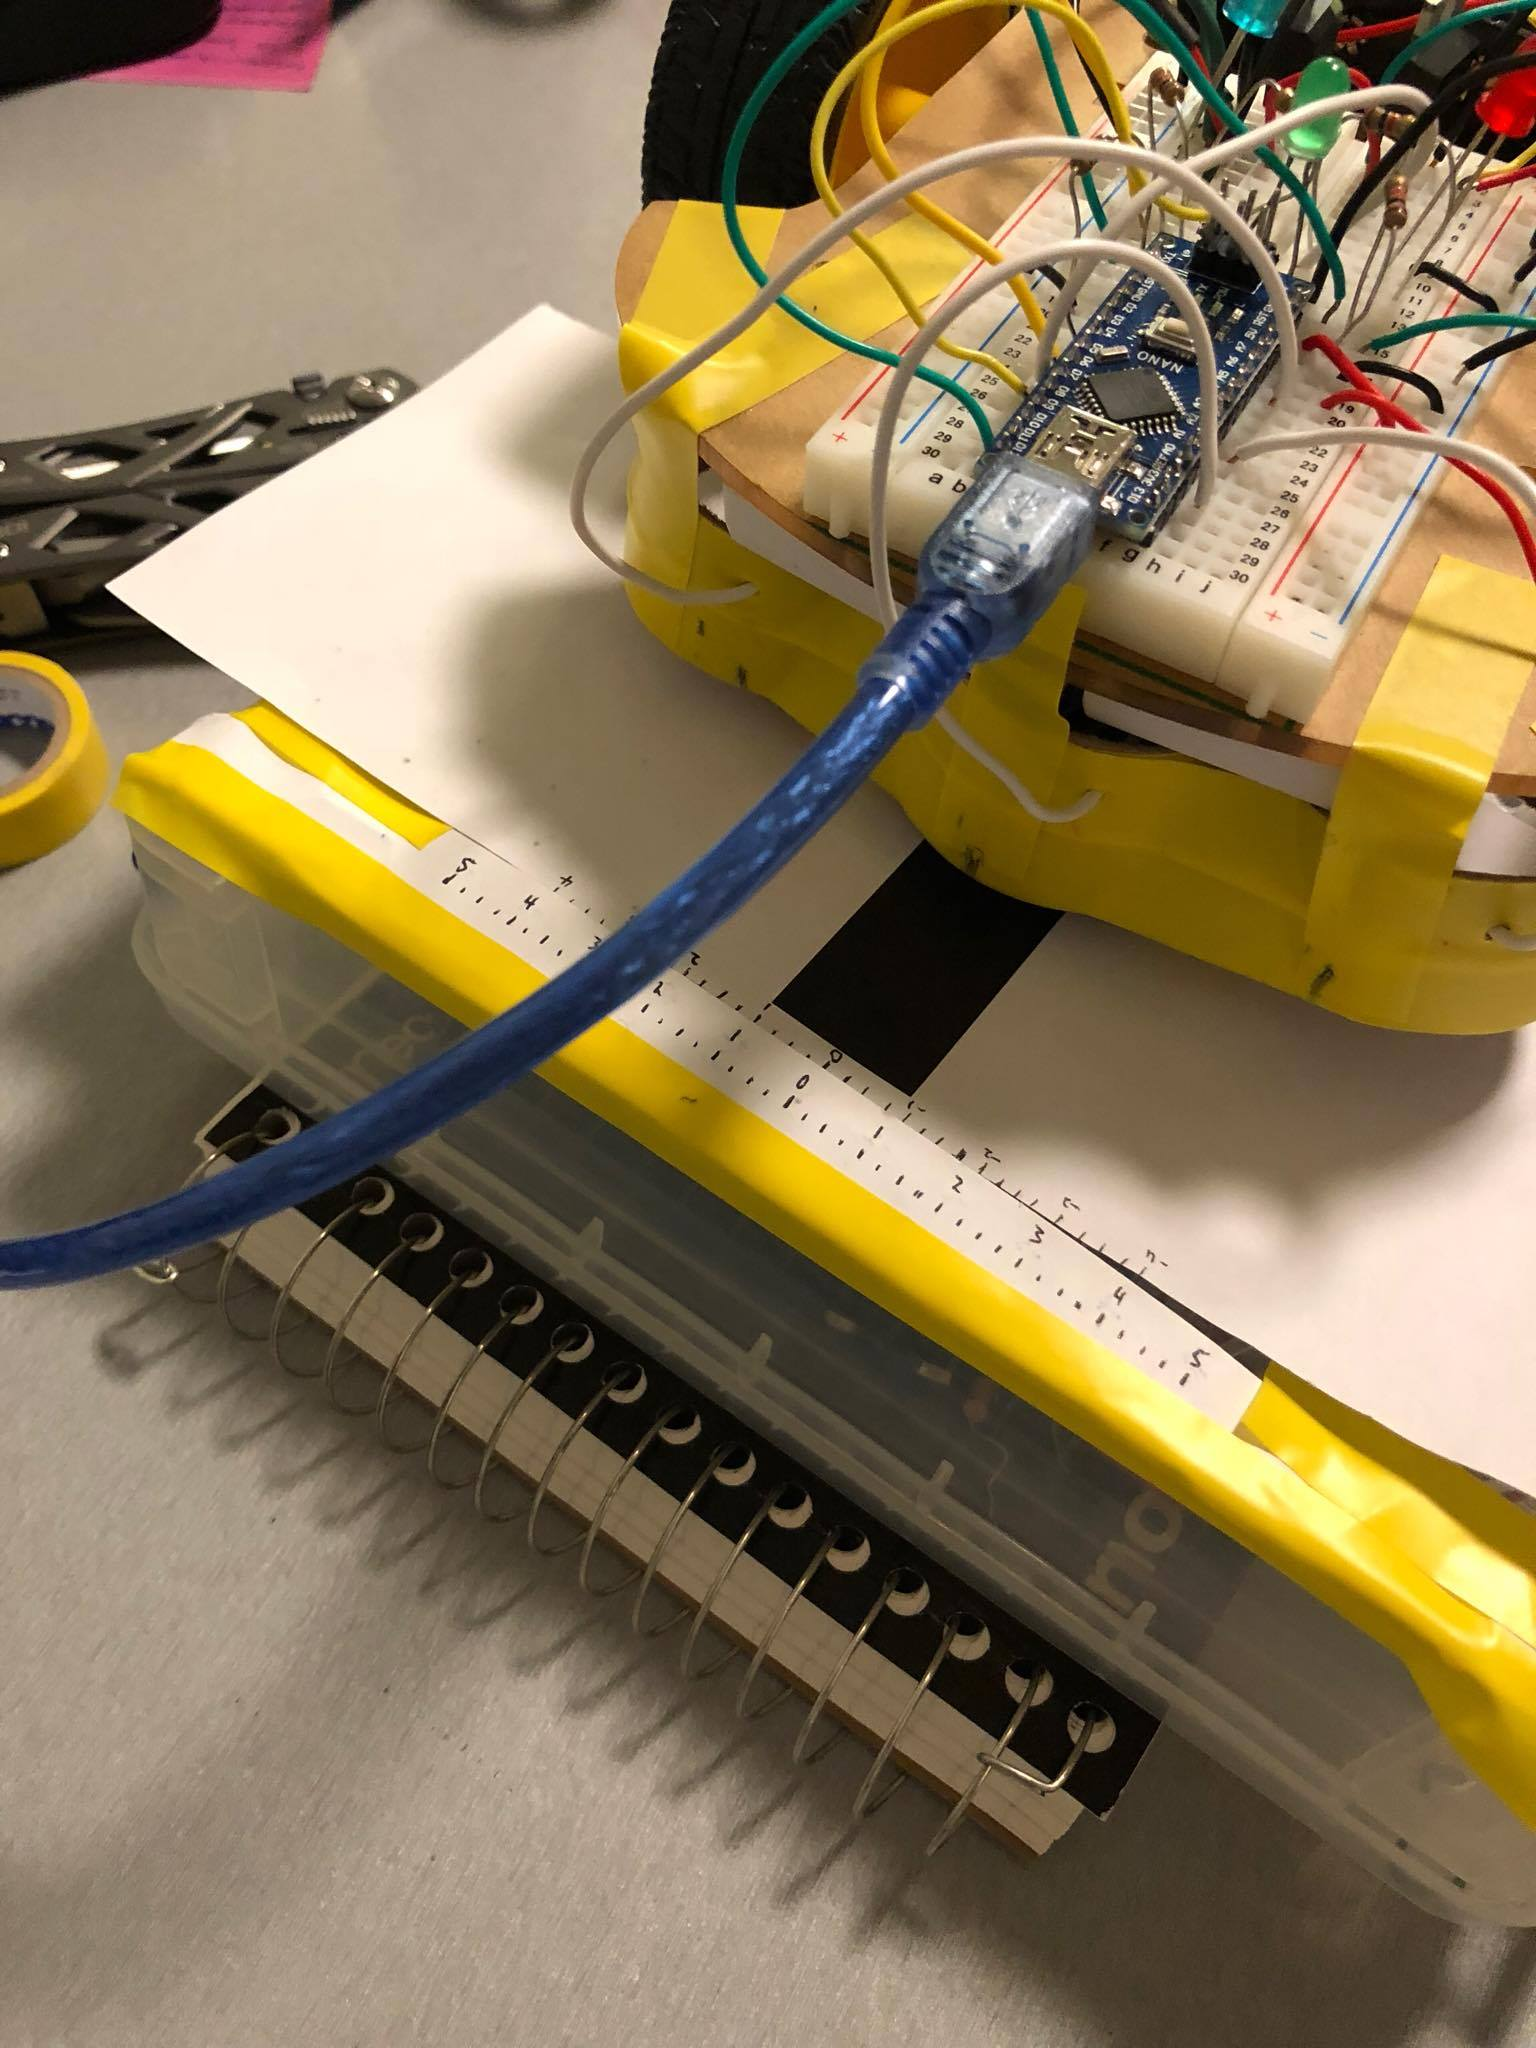
\includegraphics[width=1\columnwidth, keepaspectratio]{TestProcedure_Ruler.jpg}
					\caption{Sliding and Stationary Ruler}
					\label{fig:procedureRuler}
				\end{subfigure}
				
				\caption{Figure \ref{fig:procedureRig} shows how the car was suspended above the ruler. Figure \ref{fig:procedureRuler} shows both rulers; the stationary ruler with a range of \rpm$5cm$ and the sliding ruler with a range of \rpm$4cm$.}
			}
		\end{figure}
		
		\subsectionTitle{How We Conducted the Test}

		\textTestConduction \\ \vspace{1em}
		
		\subsectionTitle{How We Analyzed the Test Data}

		\textTestAnalysis \\ \vspace{1em}
		
		\subsectionTitle{How We Interpreted the Data}

		\textTestInterpretation \\ \vspace{1em}
		

\begin{figure*}[!B]
	\centering{
		\centering{\textbf{Raw Readings From Sensors}\par\medskip}
		\begin{subfigure}{\columnwidth}
			\centering
			\begin{tikzpicture}[
			every node/.style={text=black},
			fdesc/.default=1
			]
			
			\pgfplotsset{
				width=2.5in,
				height=2.5in,
				legend style={font=\footnotesize}
			}
			\begin{axis}[
			xlabel={Distance from Line, $cm$ ($centimeters$).},
			ylabel={Sensor Reading, $value$ ($arb.$).},
			xmin=-2, xmax=2,
			xtick distance=1,
			ymin=0, ymax=1000,
			ytick distance=200,
			]
			
			%% Marks %%
			\addplot [
			color=black,
			mark=*,
			mark options={fill=black},
			mark size=1pt
			] table [col sep=comma, y=f, x=d]{sensorsRaw.csv};
			\end{axis}
			\end{tikzpicture}
			\caption{Front Sensor}
			\vspace{0.5em}
			\label{graph:sRawFront}
		\end{subfigure}\\
		\begin{subfigure}{\columnwidth}
			\centering
			\begin{tikzpicture}[
			every node/.style={text=black},
			fdesc/.default=1
			]
			
			\pgfplotsset{
				width=2.5in,
				height=2.5in,
				legend style={font=\footnotesize}
			}
			\begin{axis}[
			xlabel={Distance from Line, $cm$ ($centimeters$).},
			ylabel={Sensor Reading, $value$ ($arb.$).},
			xmin=-2, xmax=2,
			xtick distance=1,
			ymin=0, ymax=1000,
			ytick distance=200,
			]
			
			\addplot [
			color=black,
			mark=*,
			mark options={fill=black},
			mark size=1pt
			] table [col sep=comma, y=l, x=d]{sensorsRaw.csv};
			\end{axis}
			\end{tikzpicture}
			\caption{Left Sensor}
			\label{graph:sRawLeft}
		\end{subfigure}\hfill
		\begin{subfigure}{\columnwidth}
			\centering
			\begin{tikzpicture}[
			every node/.style={text=black},
			fdesc/.default=1
			]
			
			\pgfplotsset{
				width=2.5in,
				height=2.5in,
				legend style={font=\footnotesize}
			}
			\begin{axis}[
			xlabel={Distance from Line, $cm$ ($centimeters$).},
			ylabel={Sensor Reading, $value$ ($arb.$).},
			xmin=-2, xmax=2,
			xtick distance=1,
			ymin=0, ymax=1000,
			ytick distance=200,
			]
			
			%% Marks %%
			\addplot [
			color=black,
			mark=*,
			mark options={fill=black},
			mark size=1pt
			] table [col sep=comma, y=r, x=d]{sensorsRaw.csv};
			\end{axis}
			\end{tikzpicture}
			\caption{Right Sensor}
			\label{graph:sRawRight}
		\end{subfigure}
		\caption{\textbf{Raw readings from the IR sensor, IR phototransistor combinations used on our path-following robot.} From the graphs, the value of the maximum readings range from about $400$ for Graph \ref{graph:sMappedRight} to about $600$ for Graph \ref{graph:sMappedLeft}. Also worth noting is that the sensors each reach trend down to a global minimum of around $0cm$ when moving from \rpm$1cm$ to the black line.}
	}
	\label{graph:sRaw}
\end{figure*}

		\sectionTitle{Results and Discussion}
			
			\subsectionTitle{Test Discussion}

			\textTestDiscussion \\ \vspace{1em}
			
			\subsectionTitle{Race Day Results}

			\textRaceResults \\ \vspace{1em}
			
		\sectionTitle{Conclusions and Future Work}
			
		\textConclusions \\ \vspace{1em}
		\textFutureWork \\ \vspace{1em}
			
		\sectionTitle{References}
			
		\textReferences \\ \vspace{1em}
		\printbibliography

	\end{flushleft}
	
	

		\begin{figure*}
		\centering{
			
			\centering{\textbf{Adjusted and Mapped From Sensors}\par\medskip}
					
			\begin{subfigure}{\columnwidth}
				\centering
				\begin{tikzpicture}[
				every node/.style={text=black},
				fdesc/.default=1
				]
				
				\pgfplotsset{
					width=2.5in,
					height=2.5in,
					legend style={font=\footnotesize}
				}
				\begin{axis}[
				xlabel={Distance from Line, $cm$ ($centimeters$).},
				ylabel={Adjusted Sensor Reading, $value$ ($arb.$).},
				xmin=-1, xmax=1,
				xtick distance=0.5,
				ymin=0, ymax=1,
				ytick distance=0.2,
				]
				
				%% Marks %%
				\addplot [
				color=black,
				mark=*,
				mark options={fill=black},
				mark size=1pt
				] table [col sep=comma, y=fr, x=d]{sensorsMapped.csv};
				
				\addplot [
				color=blue,
				mark=*,
				mark options={fill=blue},
				mark size=1pt
				] table [col sep=comma, y=fm, x=d]{sensorsMapped.csv};
				
				\end{axis}
				\end{tikzpicture}
				\caption{Front Sensor}
				\vspace{0.5em}
				\label{graph:sMappedFront}
			\end{subfigure}\\%
			\begin{subfigure}{\columnwidth}
				\centering
				\begin{tikzpicture}[
				every node/.style={text=black},
				fdesc/.default=1
				]
				
				\pgfplotsset{
					width=2.5in,
					height=2.5in,
					legend style={font=\footnotesize}
				}
				\begin{axis}[
				xlabel={Distance from Line, $cm$ ($centimeters$).},
				ylabel={Adjusted Sensor Reading, $value$ ($arb.$).},
				xmin=-1, xmax=1,
				xtick distance=0.5,
				ymin=0, ymax=1,
				ytick distance=0.2,
				]
				
				\addplot [
				color=black,
				mark=*,
				mark options={fill=black},
				mark size=1pt
				] table [col sep=comma, y=lr, x=d]{sensorsMapped.csv};
			
				%% Marks %%
				\addplot [
				color=blue,
				mark=*,
				mark options={fill=blue},
				mark size=1pt
				] table [col sep=comma, y=lm, x=d]{sensorsMapped.csv};
			
				\end{axis}
				\end{tikzpicture}
				\caption{Left Sensor}
				\label{graph:sMappedLeft}
			\end{subfigure}%
			\hfill
			\begin{subfigure}{\columnwidth}
				\centering
				\begin{tikzpicture}[
				every node/.style={text=black},
				fdesc/.default=1
				]
				
				\pgfplotsset{
					width=2.5in,
					height=2.5in,
					legend style={font=\footnotesize}
				}
				\begin{axis}[
				xlabel={Distance from Line, $cm$ ($centimeters$).},
				ylabel={Adjusted Sensor Reading, $value$ ($arb.$).},
				xmin=-1, xmax=1,
				xtick distance=0.5,
				ymin=0, ymax=1,
				ytick distance=0.2,
				]
				
				%% Marks %%
				\addplot [
				color=black,
				mark=*,
				mark options={fill=black},
				mark size=1pt
				] table [col sep=comma, y=rr, x=d]{sensorsMapped.csv};

				%% Marks %%
				\addplot [
				color=blue,
				mark=*,
				mark options={fill=blue},
				mark size=1pt
				] table [col sep=comma, y=rm, x=d]{sensorsMapped.csv};
				\end{axis}
				\end{tikzpicture}
				\caption{Right Sensor}
				\label{graph:sMappedRight}
			\end{subfigure}
			\caption{\textbf{Adjusted sensor readings using a crude polynomial fit of the data from Graphs \ref{graph:sRawFront}, \ref{graph:sRawLeft}, and \ref{graph:sRawRight} with a degree $n=2$ and then mapping to expand the range across the sensors line of sight ($0$ to $1cm$).} By using a polynomial fit of the sensor reading ($y$) versus the distance from the line ($x$) and solving in terms $y$, we are able to both find the distance from our readings and preserve each sensors local minimum at $0cm$. From there, we need to adjust the values to fit our known distribution and therefore simply map it as shown. By doing this, we see that our data better fits the distribution and is able to give us more valuable information to use with our PID function as the same change in the sensor reading returns a more significant change (and accurate) change in calculated distance from the line.}
		}
		\label{graph:sMapped}
	\end{figure*}

			\begin{figure*}
			\centering{
				
			\centering{\textbf{Final Readings From Sensors}\par\medskip}
						
			\begin{tikzpicture}[
			every node/.style={text=black},
			fdesc/.default=1
			]
			
			\pgfplotsset{
				width=5in,
				height=5in,
				legend style={font=\footnotesize}
			}
			\begin{axis}[
			xlabel={Distance From Line, $cm$ ($centimeters$).},
			ylabel={Absolute Distance From Line, $cm$ ($centimeters$).},
%			xmin=-1.25, xmax=1.25,
%			xtick distance=0.5,
%			ymin=-0.08, ymax=0.07,
%			ytick distance=0.03,
			xticklabel style={
				/pgf/number format/fixed,
				/pgf/number format/precision=2
			},
			scaled x ticks=false,
			yticklabel style={
				/pgf/number format/fixed,
				/pgf/number format/precision=2
			},
			scaled y ticks=false,
			]
			
			%% Marks %%
			\addplot [
			color=blue,
			mark=*,
			mark options={fill=blue},
			mark size=0.5pt,
			] table [col sep=comma, y=m, x=d]{sensorsTest.csv};
			\addlegendentry{Actual Distance};
			
			\addplot [
			color=black,
			mark=*,
			mark options={fill=black},
			mark size=0.5pt,
			] table [col sep=comma, y=a, x=d]{sensorsTest.csv};
			\addlegendentry{Calculated Distance};
			
			\draw [name path=leftBoundLeft, dashed, red] (-2.75,0) -- (-2.75,4);
			\draw [name path=leftBoundRight, dashed, red] (-1.25,0) -- (-1.25,4);
			\addplot [red!70!white,fill opacity=.2] fill between[
			of=leftBoundLeft and leftBoundRight];

			\draw [name path=rightBoundLeft, dashed] (3,0) -- (3,4);
			\draw [name path=rightBoundRight, dashed, red] (1,0) -- (1,4);
			\addplot [red!70!white,fill opacity=.2] fill between[
			of=rightBoundLeft and rightBoundRight] ;
			
			\end{axis}
			\end{tikzpicture}
			\caption{Comparison between actual and measured distance (from our getLocation() function) between center of $2cm$ thin black line and center of robot's front sensor. The red zone in the figure represent the area for which the black line is not within the range of the left, front, or right sensors. The calculated distance for these areas is just the average value of the actual distance. Looking at this graph, the calculated distance is generally accurate to within less than half a centimeter. Most importantly, the graph slopes to a minimum from both sides, an important feature if a function is to be used for a PID controller.}
			\vspace{0.5em}
			\label{graph:sensorTest}
		}
		\end{figure*}
	
%\begin{figure}[h]
%	\centering
%	\textbf{Title}\par\medskip
%	\makebox[0pt]{\includegraphics[width=1.5\textwidth,height=2\textheight,keepaspectratio]{image.jpg}}
%	\caption{Caption}
%\end{figure}

\end{document}          
